\documentclass[twoside]{book}

% Packages required by doxygen
\usepackage{fixltx2e}
\usepackage{calc}
\usepackage{doxygen}
\usepackage[export]{adjustbox} % also loads graphicx
\usepackage{graphicx}
\usepackage[utf8]{inputenc}
\usepackage{makeidx}
\usepackage{multicol}
\usepackage{multirow}
\PassOptionsToPackage{warn}{textcomp}
\usepackage{textcomp}
\usepackage[nointegrals]{wasysym}
\usepackage[table]{xcolor}

% Font selection
\usepackage[T1]{fontenc}
\usepackage[scaled=.90]{helvet}
\usepackage{courier}
\usepackage{amssymb}
\usepackage{sectsty}
\renewcommand{\familydefault}{\sfdefault}
\allsectionsfont{%
  \fontseries{bc}\selectfont%
  \color{darkgray}%
}
\renewcommand{\DoxyLabelFont}{%
  \fontseries{bc}\selectfont%
  \color{darkgray}%
}
\newcommand{\+}{\discretionary{\mbox{\scriptsize$\hookleftarrow$}}{}{}}

% Page & text layout
\usepackage{geometry}
\geometry{%
  a4paper,%
  top=2.5cm,%
  bottom=2.5cm,%
  left=2.5cm,%
  right=2.5cm%
}
\tolerance=750
\hfuzz=15pt
\hbadness=750
\setlength{\emergencystretch}{15pt}
\setlength{\parindent}{0cm}
\setlength{\parskip}{3ex plus 2ex minus 2ex}
\makeatletter
\renewcommand{\paragraph}{%
  \@startsection{paragraph}{4}{0ex}{-1.0ex}{1.0ex}{%
    \normalfont\normalsize\bfseries\SS@parafont%
  }%
}
\renewcommand{\subparagraph}{%
  \@startsection{subparagraph}{5}{0ex}{-1.0ex}{1.0ex}{%
    \normalfont\normalsize\bfseries\SS@subparafont%
  }%
}
\makeatother

% Headers & footers
\usepackage{fancyhdr}
\pagestyle{fancyplain}
\fancyhead[LE]{\fancyplain{}{\bfseries\thepage}}
\fancyhead[CE]{\fancyplain{}{}}
\fancyhead[RE]{\fancyplain{}{\bfseries\leftmark}}
\fancyhead[LO]{\fancyplain{}{\bfseries\rightmark}}
\fancyhead[CO]{\fancyplain{}{}}
\fancyhead[RO]{\fancyplain{}{\bfseries\thepage}}
\fancyfoot[LE]{\fancyplain{}{}}
\fancyfoot[CE]{\fancyplain{}{}}
\fancyfoot[RE]{\fancyplain{}{\bfseries\scriptsize Generated by Doxygen }}
\fancyfoot[LO]{\fancyplain{}{\bfseries\scriptsize Generated by Doxygen }}
\fancyfoot[CO]{\fancyplain{}{}}
\fancyfoot[RO]{\fancyplain{}{}}
\renewcommand{\footrulewidth}{0.4pt}
\renewcommand{\chaptermark}[1]{%
  \markboth{#1}{}%
}
\renewcommand{\sectionmark}[1]{%
  \markright{\thesection\ #1}%
}

% Indices & bibliography
\usepackage{natbib}
\usepackage[titles]{tocloft}
\setcounter{tocdepth}{3}
\setcounter{secnumdepth}{5}
\makeindex

% Hyperlinks (required, but should be loaded last)
\usepackage{ifpdf}
\ifpdf
  \usepackage[pdftex,pagebackref=true]{hyperref}
\else
  \usepackage[ps2pdf,pagebackref=true]{hyperref}
\fi
\hypersetup{%
  colorlinks=true,%
  linkcolor=blue,%
  citecolor=blue,%
  unicode%
}

% Custom commands
\newcommand{\clearemptydoublepage}{%
  \newpage{\pagestyle{empty}\cleardoublepage}%
}

\usepackage{caption}
\captionsetup{labelsep=space,justification=centering,font={bf},singlelinecheck=off,skip=4pt,position=top}

%===== C O N T E N T S =====

\begin{document}

% Titlepage & ToC
\hypersetup{pageanchor=false,
             bookmarksnumbered=true,
             pdfencoding=unicode
            }
\pagenumbering{alph}
\begin{titlepage}
\vspace*{7cm}
\begin{center}%
{\Large My Project }\\
\vspace*{1cm}
{\large Generated by Doxygen 1.8.13}\\
\end{center}
\end{titlepage}
\clearemptydoublepage
\pagenumbering{roman}
\tableofcontents
\clearemptydoublepage
\pagenumbering{arabic}
\hypersetup{pageanchor=true}

%--- Begin generated contents ---
\chapter{Namespace Index}
\section{Namespace List}
Here is a list of all documented namespaces with brief descriptions\+:\begin{DoxyCompactList}
\item\contentsline{section}{\hyperlink{namespacechecking__argument}{checking\+\_\+argument} }{\pageref{namespacechecking__argument}}{}
\item\contentsline{section}{\hyperlink{namespaceconformation}{conformation} }{\pageref{namespaceconformation}}{}
\item\contentsline{section}{\hyperlink{namespacemain}{main} }{\pageref{namespacemain}}{}
\item\contentsline{section}{\hyperlink{namespacemonte__carlo}{monte\+\_\+carlo} }{\pageref{namespacemonte__carlo}}{}
\end{DoxyCompactList}

\chapter{Hierarchical Index}
\section{Class Hierarchy}
This inheritance list is sorted roughly, but not completely, alphabetically\+:\begin{DoxyCompactList}
\item \contentsline{section}{Movement.\+Movement}{\pageref{classMovement_1_1Movement}}{}
\begin{DoxyCompactList}
\item \contentsline{section}{Corner\+\_\+moves.\+Corner\+\_\+moves}{\pageref{classCorner__moves_1_1Corner__moves}}{}
\item \contentsline{section}{Crankshaft\+\_\+moves.\+Crankshaft\+\_\+moves}{\pageref{classCrankshaft__moves_1_1Crankshaft__moves}}{}
\item \contentsline{section}{End\+\_\+moves.\+End\+\_\+moves}{\pageref{classEnd__moves_1_1End__moves}}{}
\item \contentsline{section}{Pull\+\_\+moves.\+Pull\+\_\+moves}{\pageref{classPull__moves_1_1Pull__moves}}{}
\end{DoxyCompactList}
\item \contentsline{section}{Residu.\+Residu}{\pageref{classResidu_1_1Residu}}{}
\end{DoxyCompactList}

\chapter{Class Index}
\section{Class List}
Here are the classes, structs, unions and interfaces with brief descriptions\+:\begin{DoxyCompactList}
\item\contentsline{section}{\hyperlink{classCorner__moves_1_1Corner__moves}{Corner\+\_\+moves.\+Corner\+\_\+moves} }{\pageref{classCorner__moves_1_1Corner__moves}}{}
\item\contentsline{section}{\hyperlink{classCrankshaft__moves_1_1Crankshaft__moves}{Crankshaft\+\_\+moves.\+Crankshaft\+\_\+moves} }{\pageref{classCrankshaft__moves_1_1Crankshaft__moves}}{}
\item\contentsline{section}{\hyperlink{classEnd__moves_1_1End__moves}{End\+\_\+moves.\+End\+\_\+moves} }{\pageref{classEnd__moves_1_1End__moves}}{}
\item\contentsline{section}{\hyperlink{classMovement_1_1Movement}{Movement.\+Movement} }{\pageref{classMovement_1_1Movement}}{}
\item\contentsline{section}{\hyperlink{classPull__moves_1_1Pull__moves}{Pull\+\_\+moves.\+Pull\+\_\+moves} }{\pageref{classPull__moves_1_1Pull__moves}}{}
\item\contentsline{section}{\hyperlink{classResidu_1_1Residu}{Residu.\+Residu} }{\pageref{classResidu_1_1Residu}}{}
\end{DoxyCompactList}

\chapter{Namespace Documentation}
\hypertarget{namespacecheckingArgument}{}\section{checking\+Argument Namespace Reference}
\label{namespacecheckingArgument}\index{checking\+Argument@{checking\+Argument}}
\subsection*{Functions}
\begin{DoxyCompactItemize}
\item 
def \hyperlink{namespacecheckingArgument_a1d9eb47180088481295bcbe4edb1d3e9}{check\+\_\+int\+\_\+type} (rep)
\item 
def \hyperlink{namespacecheckingArgument_a5c2a1e659d8c6bad279afc69226c8077}{check\+\_\+arguments} (argv)
\end{DoxyCompactItemize}


\subsection{Detailed Description}
\begin{DoxyVerb}    Check if user enter all necessary arguments correctly.
    Otherwise, a message is sent to the user.
\end{DoxyVerb}
 

\subsection{Function Documentation}
\mbox{\Hypertarget{namespacecheckingArgument_a5c2a1e659d8c6bad279afc69226c8077}\label{namespacecheckingArgument_a5c2a1e659d8c6bad279afc69226c8077}} 
\index{checking\+Argument@{checking\+Argument}!check\+\_\+arguments@{check\+\_\+arguments}}
\index{check\+\_\+arguments@{check\+\_\+arguments}!checking\+Argument@{checking\+Argument}}
\subsubsection{\texorpdfstring{check\+\_\+arguments()}{check\_arguments()}}
{\footnotesize\ttfamily def checking\+Argument.\+check\+\_\+arguments (\begin{DoxyParamCaption}\item[{}]{argv }\end{DoxyParamCaption})}

\begin{DoxyVerb}Assign options into variable and check if
    option are correct.
\end{DoxyVerb}
 \mbox{\Hypertarget{namespacecheckingArgument_a1d9eb47180088481295bcbe4edb1d3e9}\label{namespacecheckingArgument_a1d9eb47180088481295bcbe4edb1d3e9}} 
\index{checking\+Argument@{checking\+Argument}!check\+\_\+int\+\_\+type@{check\+\_\+int\+\_\+type}}
\index{check\+\_\+int\+\_\+type@{check\+\_\+int\+\_\+type}!checking\+Argument@{checking\+Argument}}
\subsubsection{\texorpdfstring{check\+\_\+int\+\_\+type()}{check\_int\_type()}}
{\footnotesize\ttfamily def checking\+Argument.\+check\+\_\+int\+\_\+type (\begin{DoxyParamCaption}\item[{}]{rep }\end{DoxyParamCaption})}

\begin{DoxyVerb}Check if the answer can be cast into int
    and return it
\end{DoxyVerb}
 
\hypertarget{namespaceconformation}{}\section{conformation Namespace Reference}
\label{namespaceconformation}\index{conformation@{conformation}}
\subsection*{Functions}
\begin{DoxyCompactItemize}
\item 
def \hyperlink{namespaceconformation_a68e0c087ab604cbc37a7fe9a27622d8c}{vshd\+\_\+move} (index, structure\+\_\+grid, residues)
\item 
\mbox{\Hypertarget{namespaceconformation_aff463b8b684c4af25a3016b5e9bde9a7}\label{namespaceconformation_aff463b8b684c4af25a3016b5e9bde9a7}} 
def {\bfseries pullmoves\+\_\+move} (residu, structure\+\_\+grid)
\item 
\mbox{\Hypertarget{namespaceconformation_aff776064950617ef8272323343ef9a95}\label{namespaceconformation_aff776064950617ef8272323343ef9a95}} 
def {\bfseries mixe\+\_\+move} (residu, structure\+\_\+grid)
\end{DoxyCompactItemize}


\subsection{Detailed Description}
\begin{DoxyVerb}    Define different movement possible according to user's choice.
    Then, launch the most appropriate movement.
\end{DoxyVerb}
 

\subsection{Function Documentation}
\mbox{\Hypertarget{namespaceconformation_a68e0c087ab604cbc37a7fe9a27622d8c}\label{namespaceconformation_a68e0c087ab604cbc37a7fe9a27622d8c}} 
\index{conformation@{conformation}!vshd\+\_\+move@{vshd\+\_\+move}}
\index{vshd\+\_\+move@{vshd\+\_\+move}!conformation@{conformation}}
\subsubsection{\texorpdfstring{vshd\+\_\+move()}{vshd\_move()}}
{\footnotesize\ttfamily def conformation.\+vshd\+\_\+move (\begin{DoxyParamCaption}\item[{}]{index,  }\item[{}]{structure\+\_\+grid,  }\item[{}]{residues }\end{DoxyParamCaption})}

\begin{DoxyVerb}Launch a VSHD movement according to the random residu.
    Return a list with the new lattice and  the new residues object
\end{DoxyVerb}
 
\hypertarget{namespacemain}{}\section{main Namespace Reference}
\label{namespacemain}\index{main@{main}}
\subsection*{Functions}
\begin{DoxyCompactItemize}
\item 
def \hyperlink{namespacemain_aa6f8a1443820135b3cf84d9bafcc0028}{display} (residues, energy, idx)
\end{DoxyCompactItemize}
\subsection*{Variables}
\begin{DoxyCompactItemize}
\item 
\mbox{\Hypertarget{namespacemain_a3c60151b99b469323d8c15116db80817}\label{namespacemain_a3c60151b99b469323d8c15116db80817}} 
{\bfseries tic} = time.\+time()
\item 
\mbox{\Hypertarget{namespacemain_ab56df29b0534dd6fbd128d54225bee86}\label{namespacemain_ab56df29b0534dd6fbd128d54225bee86}} 
list {\bfseries replicates} = \mbox{[}None\mbox{]} $\ast$ c\+A.\+R\+E\+P\+L\+I\+CA
\item 
\mbox{\Hypertarget{namespacemain_a9c81977c283643c4d0c96b128722e771}\label{namespacemain_a9c81977c283643c4d0c96b128722e771}} 
tuple {\bfseries shift} = (c\+A.\+T\+E\+M\+P\+E\+R\+A\+T\+U\+RE -\/ 220) / c\+A.\+R\+E\+P\+L\+I\+CA
\item 
\mbox{\Hypertarget{namespacemain_aa03ea582ff8e07a50e1d850a94da8247}\label{namespacemain_aa03ea582ff8e07a50e1d850a94da8247}} 
{\bfseries residues}
\item 
\mbox{\Hypertarget{namespacemain_a67a4a2ee96191c0257e4744c29dacebf}\label{namespacemain_a67a4a2ee96191c0257e4744c29dacebf}} 
{\bfseries structure\+\_\+grid}
\item 
\mbox{\Hypertarget{namespacemain_a42e4c3ac704d1a088d18d3e7c32cca23}\label{namespacemain_a42e4c3ac704d1a088d18d3e7c32cca23}} 
{\bfseries toc} = time.\+time()
\end{DoxyCompactItemize}


\subsection{Detailed Description}
\begin{DoxyVerb}REMC script

Usage:
  main.py -s <seq> -e <x> -m <move>
  main.py -s <seq> -e <x> -m <move> [-p <nb_steps>] [-t <temp>] [-r <nb_rep>]

Options:
  -h --help                  help
  --version                  version of the script
  -s --sequence = seq        write the sequence according to HP model
  -e --energy = x            write the mminimum energy to reach
  -m --movement = move       VSHD, PULLMOVES or MIXE
  -p --steps = nb_steps      the maximum steps [default: 500]
  -t --temperature = temp    the minimal temperature [default: 160]
  -r --replica = nb_rep      number of replica [default: 5]
\end{DoxyVerb}
 

\subsection{Function Documentation}
\mbox{\Hypertarget{namespacemain_aa6f8a1443820135b3cf84d9bafcc0028}\label{namespacemain_aa6f8a1443820135b3cf84d9bafcc0028}} 
\index{main@{main}!display@{display}}
\index{display@{display}!main@{main}}
\subsubsection{\texorpdfstring{display()}{display()}}
{\footnotesize\ttfamily def main.\+display (\begin{DoxyParamCaption}\item[{}]{residues,  }\item[{}]{energy,  }\item[{}]{idx }\end{DoxyParamCaption})}

\begin{DoxyVerb}Plot the conformation of each replica in 3D with matplotlib
    @param residues: A list of residu object
    @param idx: The index of the rpelica for the title
\end{DoxyVerb}
 
\chapter{Class Documentation}
\hypertarget{classCorner__moves_1_1Corner__moves}{}\section{Corner\+\_\+moves.\+Corner\+\_\+moves Class Reference}
\label{classCorner__moves_1_1Corner__moves}\index{Corner\+\_\+moves.\+Corner\+\_\+moves@{Corner\+\_\+moves.\+Corner\+\_\+moves}}


Inheritance diagram for Corner\+\_\+moves.\+Corner\+\_\+moves\+:
\nopagebreak
\begin{figure}[H]
\begin{center}
\leavevmode
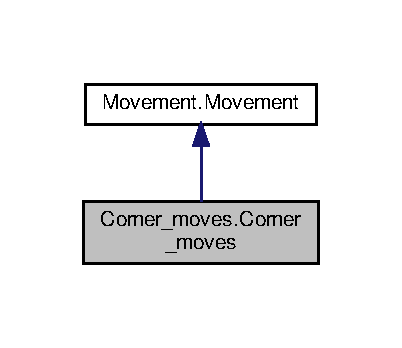
\includegraphics[width=193pt]{classCorner__moves_1_1Corner__moves__inherit__graph}
\end{center}
\end{figure}


Collaboration diagram for Corner\+\_\+moves.\+Corner\+\_\+moves\+:
\nopagebreak
\begin{figure}[H]
\begin{center}
\leavevmode
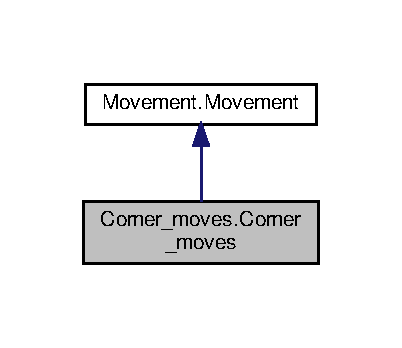
\includegraphics[width=193pt]{classCorner__moves_1_1Corner__moves__coll__graph}
\end{center}
\end{figure}
\subsection*{Public Member Functions}
\begin{DoxyCompactItemize}
\item 
def \hyperlink{classCorner__moves_1_1Corner__moves_aa6b7b51aa871e3b5c2cdc5ed14fe5706}{mutation} (self, structure\+\_\+grid)
\item 
def \hyperlink{classCorner__moves_1_1Corner__moves_af74a6a204959ce19e1f9a10a8b4c8000}{\+\_\+\+\_\+init\+\_\+\+\_\+} (self, res, i)
\end{DoxyCompactItemize}
\subsection*{Public Attributes}
\begin{DoxyCompactItemize}
\item 
\mbox{\Hypertarget{classCorner__moves_1_1Corner__moves_a306f0fe66fe24b76781a5e24128d8fb6}\label{classCorner__moves_1_1Corner__moves_a306f0fe66fe24b76781a5e24128d8fb6}} 
{\bfseries residu}
\end{DoxyCompactItemize}


\subsection{Detailed Description}
\begin{DoxyVerb}To be possible, the two connected neighbours of some residue i must
    be mutually adjacent to another, unoccupied position on the lattice.
\end{DoxyVerb}
 

\subsection{Constructor \& Destructor Documentation}
\mbox{\Hypertarget{classCorner__moves_1_1Corner__moves_af74a6a204959ce19e1f9a10a8b4c8000}\label{classCorner__moves_1_1Corner__moves_af74a6a204959ce19e1f9a10a8b4c8000}} 
\index{Corner\+\_\+moves\+::\+Corner\+\_\+moves@{Corner\+\_\+moves\+::\+Corner\+\_\+moves}!\+\_\+\+\_\+init\+\_\+\+\_\+@{\+\_\+\+\_\+init\+\_\+\+\_\+}}
\index{\+\_\+\+\_\+init\+\_\+\+\_\+@{\+\_\+\+\_\+init\+\_\+\+\_\+}!Corner\+\_\+moves\+::\+Corner\+\_\+moves@{Corner\+\_\+moves\+::\+Corner\+\_\+moves}}
\subsubsection{\texorpdfstring{\+\_\+\+\_\+init\+\_\+\+\_\+()}{\_\_init\_\_()}}
{\footnotesize\ttfamily def Corner\+\_\+moves.\+Corner\+\_\+moves.\+\_\+\+\_\+init\+\_\+\+\_\+ (\begin{DoxyParamCaption}\item[{}]{self,  }\item[{}]{res,  }\item[{}]{i }\end{DoxyParamCaption})}

\begin{DoxyVerb}Initialize the object Corner_moves
    :param res: Residu object
    :param   i: index of the Residu object
\end{DoxyVerb}
 

\subsection{Member Function Documentation}
\mbox{\Hypertarget{classCorner__moves_1_1Corner__moves_aa6b7b51aa871e3b5c2cdc5ed14fe5706}\label{classCorner__moves_1_1Corner__moves_aa6b7b51aa871e3b5c2cdc5ed14fe5706}} 
\index{Corner\+\_\+moves\+::\+Corner\+\_\+moves@{Corner\+\_\+moves\+::\+Corner\+\_\+moves}!mutation@{mutation}}
\index{mutation@{mutation}!Corner\+\_\+moves\+::\+Corner\+\_\+moves@{Corner\+\_\+moves\+::\+Corner\+\_\+moves}}
\subsubsection{\texorpdfstring{mutation()}{mutation()}}
{\footnotesize\ttfamily def Corner\+\_\+moves.\+Corner\+\_\+moves.\+mutation (\begin{DoxyParamCaption}\item[{}]{self,  }\item[{}]{structure\+\_\+grid }\end{DoxyParamCaption})}

\begin{DoxyVerb}Search the unoccupied position for the movement
    Return the solution or None if the movement is not possible
\end{DoxyVerb}
 

The documentation for this class was generated from the following file\+:\begin{DoxyCompactItemize}
\item 
Corner\+\_\+moves.\+py\end{DoxyCompactItemize}

\hypertarget{classCrankshaft__moves_1_1Crankshaft__moves}{}\section{Crankshaft\+\_\+moves.\+Crankshaft\+\_\+moves Class Reference}
\label{classCrankshaft__moves_1_1Crankshaft__moves}\index{Crankshaft\+\_\+moves.\+Crankshaft\+\_\+moves@{Crankshaft\+\_\+moves.\+Crankshaft\+\_\+moves}}


Inheritance diagram for Crankshaft\+\_\+moves.\+Crankshaft\+\_\+moves\+:
\nopagebreak
\begin{figure}[H]
\begin{center}
\leavevmode
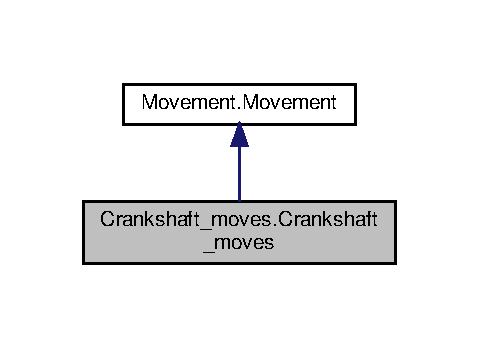
\includegraphics[width=230pt]{classCrankshaft__moves_1_1Crankshaft__moves__inherit__graph}
\end{center}
\end{figure}


Collaboration diagram for Crankshaft\+\_\+moves.\+Crankshaft\+\_\+moves\+:
\nopagebreak
\begin{figure}[H]
\begin{center}
\leavevmode
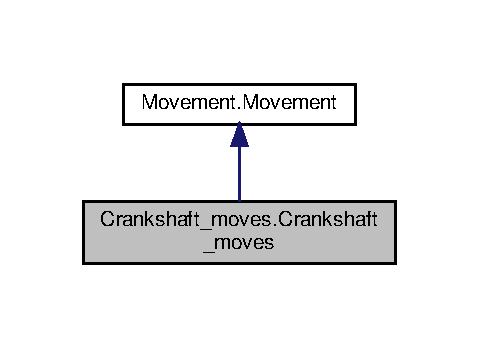
\includegraphics[width=230pt]{classCrankshaft__moves_1_1Crankshaft__moves__coll__graph}
\end{center}
\end{figure}
\subsection*{Public Member Functions}
\begin{DoxyCompactItemize}
\item 
def \hyperlink{classCrankshaft__moves_1_1Crankshaft__moves_a9373405d3071eedd7d35a92ecd1aa3af}{mutation} (self, structure\+\_\+grid)
\item 
def \hyperlink{classCrankshaft__moves_1_1Crankshaft__moves_a5f336d38f0adee71bf8d6c9a9c0b4d7e}{\+\_\+\+\_\+init\+\_\+\+\_\+} (self, res, i)
\end{DoxyCompactItemize}
\subsection*{Public Attributes}
\begin{DoxyCompactItemize}
\item 
\mbox{\Hypertarget{classCrankshaft__moves_1_1Crankshaft__moves_a88f703bb354d88edc6eb75b25179ecd7}\label{classCrankshaft__moves_1_1Crankshaft__moves_a88f703bb354d88edc6eb75b25179ecd7}} 
{\bfseries residu}
\end{DoxyCompactItemize}


\subsection{Detailed Description}
\begin{DoxyVerb}To be possible, residue i is part of a u-shaped bend in the chain which
    involves a 180° rotation of a u-shaped structure consisting
    of four connected neighbours.
\end{DoxyVerb}
 

\subsection{Constructor \& Destructor Documentation}
\mbox{\Hypertarget{classCrankshaft__moves_1_1Crankshaft__moves_a5f336d38f0adee71bf8d6c9a9c0b4d7e}\label{classCrankshaft__moves_1_1Crankshaft__moves_a5f336d38f0adee71bf8d6c9a9c0b4d7e}} 
\index{Crankshaft\+\_\+moves\+::\+Crankshaft\+\_\+moves@{Crankshaft\+\_\+moves\+::\+Crankshaft\+\_\+moves}!\+\_\+\+\_\+init\+\_\+\+\_\+@{\+\_\+\+\_\+init\+\_\+\+\_\+}}
\index{\+\_\+\+\_\+init\+\_\+\+\_\+@{\+\_\+\+\_\+init\+\_\+\+\_\+}!Crankshaft\+\_\+moves\+::\+Crankshaft\+\_\+moves@{Crankshaft\+\_\+moves\+::\+Crankshaft\+\_\+moves}}
\subsubsection{\texorpdfstring{\+\_\+\+\_\+init\+\_\+\+\_\+()}{\_\_init\_\_()}}
{\footnotesize\ttfamily def Crankshaft\+\_\+moves.\+Crankshaft\+\_\+moves.\+\_\+\+\_\+init\+\_\+\+\_\+ (\begin{DoxyParamCaption}\item[{}]{self,  }\item[{}]{res,  }\item[{}]{i }\end{DoxyParamCaption})}

\begin{DoxyVerb}Initialize the object Crankshaft_moves
    :param res: Residu object
    :param   i: index of the Residu object
\end{DoxyVerb}
 

\subsection{Member Function Documentation}
\mbox{\Hypertarget{classCrankshaft__moves_1_1Crankshaft__moves_a9373405d3071eedd7d35a92ecd1aa3af}\label{classCrankshaft__moves_1_1Crankshaft__moves_a9373405d3071eedd7d35a92ecd1aa3af}} 
\index{Crankshaft\+\_\+moves\+::\+Crankshaft\+\_\+moves@{Crankshaft\+\_\+moves\+::\+Crankshaft\+\_\+moves}!mutation@{mutation}}
\index{mutation@{mutation}!Crankshaft\+\_\+moves\+::\+Crankshaft\+\_\+moves@{Crankshaft\+\_\+moves\+::\+Crankshaft\+\_\+moves}}
\subsubsection{\texorpdfstring{mutation()}{mutation()}}
{\footnotesize\ttfamily def Crankshaft\+\_\+moves.\+Crankshaft\+\_\+moves.\+mutation (\begin{DoxyParamCaption}\item[{}]{self,  }\item[{}]{structure\+\_\+grid }\end{DoxyParamCaption})}

\begin{DoxyVerb}Search if the residu i is part of a u-shaped then search the rotation
    Return the 2 free neighbour in a list
\end{DoxyVerb}
 

The documentation for this class was generated from the following file\+:\begin{DoxyCompactItemize}
\item 
Crankshaft\+\_\+moves.\+py\end{DoxyCompactItemize}

\hypertarget{classEnd__moves_1_1End__moves}{}\section{End\+\_\+moves.\+End\+\_\+moves Class Reference}
\label{classEnd__moves_1_1End__moves}\index{End\+\_\+moves.\+End\+\_\+moves@{End\+\_\+moves.\+End\+\_\+moves}}


Inheritance diagram for End\+\_\+moves.\+End\+\_\+moves\+:
\nopagebreak
\begin{figure}[H]
\begin{center}
\leavevmode
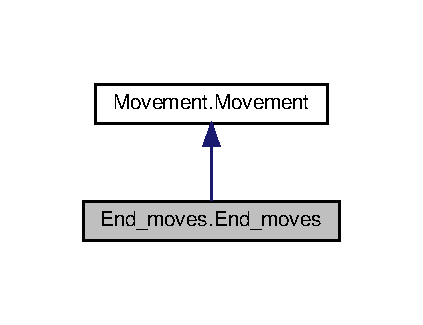
\includegraphics[width=203pt]{classEnd__moves_1_1End__moves__inherit__graph}
\end{center}
\end{figure}


Collaboration diagram for End\+\_\+moves.\+End\+\_\+moves\+:
\nopagebreak
\begin{figure}[H]
\begin{center}
\leavevmode
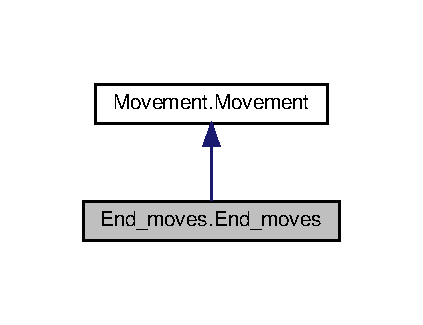
\includegraphics[width=203pt]{classEnd__moves_1_1End__moves__coll__graph}
\end{center}
\end{figure}
\subsection*{Public Member Functions}
\begin{DoxyCompactItemize}
\item 
def \hyperlink{classEnd__moves_1_1End__moves_a398d49afd0af75f9dd3306d66ab4f244}{mutation} (self, structure\+\_\+grid)
\item 
def \hyperlink{classEnd__moves_1_1End__moves_ae5788aa8e49a0569fc9c88cb3a74e722}{\+\_\+\+\_\+init\+\_\+\+\_\+} (self, res, i)
\end{DoxyCompactItemize}
\subsection*{Public Attributes}
\begin{DoxyCompactItemize}
\item 
\mbox{\Hypertarget{classEnd__moves_1_1End__moves_a1b7617746594f19259fa997839b674b4}\label{classEnd__moves_1_1End__moves_a1b7617746594f19259fa997839b674b4}} 
{\bfseries index}
\item 
\mbox{\Hypertarget{classEnd__moves_1_1End__moves_aa62e058761c54511a7f379ae0c4c8608}\label{classEnd__moves_1_1End__moves_aa62e058761c54511a7f379ae0c4c8608}} 
{\bfseries residu}
\end{DoxyCompactItemize}


\subsection{Detailed Description}
\begin{DoxyVerb}The residue is pivoted relative to its connected
    neighbour to a free position adjacent to that neighbour.
\end{DoxyVerb}
 

\subsection{Constructor \& Destructor Documentation}
\mbox{\Hypertarget{classEnd__moves_1_1End__moves_ae5788aa8e49a0569fc9c88cb3a74e722}\label{classEnd__moves_1_1End__moves_ae5788aa8e49a0569fc9c88cb3a74e722}} 
\index{End\+\_\+moves\+::\+End\+\_\+moves@{End\+\_\+moves\+::\+End\+\_\+moves}!\+\_\+\+\_\+init\+\_\+\+\_\+@{\+\_\+\+\_\+init\+\_\+\+\_\+}}
\index{\+\_\+\+\_\+init\+\_\+\+\_\+@{\+\_\+\+\_\+init\+\_\+\+\_\+}!End\+\_\+moves\+::\+End\+\_\+moves@{End\+\_\+moves\+::\+End\+\_\+moves}}
\subsubsection{\texorpdfstring{\+\_\+\+\_\+init\+\_\+\+\_\+()}{\_\_init\_\_()}}
{\footnotesize\ttfamily def End\+\_\+moves.\+End\+\_\+moves.\+\_\+\+\_\+init\+\_\+\+\_\+ (\begin{DoxyParamCaption}\item[{}]{self,  }\item[{}]{res,  }\item[{}]{i }\end{DoxyParamCaption})}

\begin{DoxyVerb}Initialize the object End_moves
    :param res: Residu object
    :param   i: index of the Residu object
\end{DoxyVerb}
 

\subsection{Member Function Documentation}
\mbox{\Hypertarget{classEnd__moves_1_1End__moves_a398d49afd0af75f9dd3306d66ab4f244}\label{classEnd__moves_1_1End__moves_a398d49afd0af75f9dd3306d66ab4f244}} 
\index{End\+\_\+moves\+::\+End\+\_\+moves@{End\+\_\+moves\+::\+End\+\_\+moves}!mutation@{mutation}}
\index{mutation@{mutation}!End\+\_\+moves\+::\+End\+\_\+moves@{End\+\_\+moves\+::\+End\+\_\+moves}}
\subsubsection{\texorpdfstring{mutation()}{mutation()}}
{\footnotesize\ttfamily def End\+\_\+moves.\+End\+\_\+moves.\+mutation (\begin{DoxyParamCaption}\item[{}]{self,  }\item[{}]{structure\+\_\+grid }\end{DoxyParamCaption})}

\begin{DoxyVerb}Search free neighbour for the residu adjacent.
    If several positions are free, on
    is chosen randomly and the residu is pivoted to this position.
\end{DoxyVerb}
 

The documentation for this class was generated from the following file\+:\begin{DoxyCompactItemize}
\item 
End\+\_\+moves.\+py\end{DoxyCompactItemize}

\hypertarget{classMovement_1_1Movement}{}\section{Movement.\+Movement Class Reference}
\label{classMovement_1_1Movement}\index{Movement.\+Movement@{Movement.\+Movement}}


Inheritance diagram for Movement.\+Movement\+:
\nopagebreak
\begin{figure}[H]
\begin{center}
\leavevmode
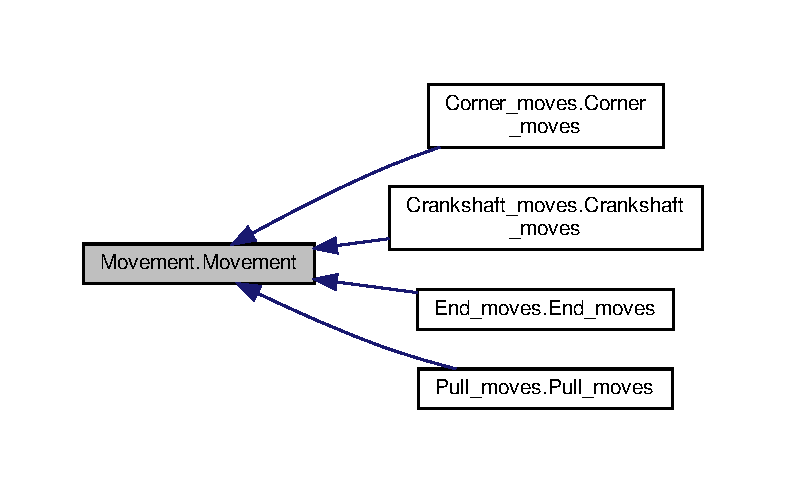
\includegraphics[width=350pt]{classMovement_1_1Movement__inherit__graph}
\end{center}
\end{figure}
\subsection*{Public Member Functions}
\begin{DoxyCompactItemize}
\item 
def \hyperlink{classMovement_1_1Movement_a9a5855cfc798666c18371ea030ae54a7}{count\+Bonds} (self, structure\+\_\+grid, residues)
\item 
def \hyperlink{classMovement_1_1Movement_ac3dec9f23b8e853ac5101535ee804767}{change\+One\+Residu} (self, structure\+\_\+grid, residues, random\+\_\+neighbour)
\item 
def \hyperlink{classMovement_1_1Movement_a9052fb0d7d5328a995abee94111d9fcc}{change\+Two\+Residues} (self, structure\+\_\+grid, residues, random\+\_\+neighbour)
\item 
def \hyperlink{classMovement_1_1Movement_a30e499b5ab0257aac5ee77dc24c161b5}{\+\_\+\+\_\+init\+\_\+\+\_\+} (self, i)
\end{DoxyCompactItemize}
\subsection*{Public Attributes}
\begin{DoxyCompactItemize}
\item 
\mbox{\Hypertarget{classMovement_1_1Movement_a8972b130eb57f4921311faf370d11c79}\label{classMovement_1_1Movement_a8972b130eb57f4921311faf370d11c79}} 
{\bfseries index}
\end{DoxyCompactItemize}


\subsection{Detailed Description}
\begin{DoxyVerb}Mother class of all movements.
\end{DoxyVerb}
 

\subsection{Constructor \& Destructor Documentation}
\mbox{\Hypertarget{classMovement_1_1Movement_a30e499b5ab0257aac5ee77dc24c161b5}\label{classMovement_1_1Movement_a30e499b5ab0257aac5ee77dc24c161b5}} 
\index{Movement\+::\+Movement@{Movement\+::\+Movement}!\+\_\+\+\_\+init\+\_\+\+\_\+@{\+\_\+\+\_\+init\+\_\+\+\_\+}}
\index{\+\_\+\+\_\+init\+\_\+\+\_\+@{\+\_\+\+\_\+init\+\_\+\+\_\+}!Movement\+::\+Movement@{Movement\+::\+Movement}}
\subsubsection{\texorpdfstring{\+\_\+\+\_\+init\+\_\+\+\_\+()}{\_\_init\_\_()}}
{\footnotesize\ttfamily def Movement.\+Movement.\+\_\+\+\_\+init\+\_\+\+\_\+ (\begin{DoxyParamCaption}\item[{}]{self,  }\item[{}]{i }\end{DoxyParamCaption})}

\begin{DoxyVerb}Initialize the object Movement
    :param   i: index of the Residu object
\end{DoxyVerb}
 

\subsection{Member Function Documentation}
\mbox{\Hypertarget{classMovement_1_1Movement_ac3dec9f23b8e853ac5101535ee804767}\label{classMovement_1_1Movement_ac3dec9f23b8e853ac5101535ee804767}} 
\index{Movement\+::\+Movement@{Movement\+::\+Movement}!change\+One\+Residu@{change\+One\+Residu}}
\index{change\+One\+Residu@{change\+One\+Residu}!Movement\+::\+Movement@{Movement\+::\+Movement}}
\subsubsection{\texorpdfstring{change\+One\+Residu()}{changeOneResidu()}}
{\footnotesize\ttfamily def Movement.\+Movement.\+change\+One\+Residu (\begin{DoxyParamCaption}\item[{}]{self,  }\item[{}]{structure\+\_\+grid,  }\item[{}]{residues,  }\item[{}]{random\+\_\+neighbour }\end{DoxyParamCaption})}

\begin{DoxyVerb}Change the conformation of one residu.
    Return the new conformation and residues obejct modified.
\end{DoxyVerb}
 \mbox{\Hypertarget{classMovement_1_1Movement_a9052fb0d7d5328a995abee94111d9fcc}\label{classMovement_1_1Movement_a9052fb0d7d5328a995abee94111d9fcc}} 
\index{Movement\+::\+Movement@{Movement\+::\+Movement}!change\+Two\+Residues@{change\+Two\+Residues}}
\index{change\+Two\+Residues@{change\+Two\+Residues}!Movement\+::\+Movement@{Movement\+::\+Movement}}
\subsubsection{\texorpdfstring{change\+Two\+Residues()}{changeTwoResidues()}}
{\footnotesize\ttfamily def Movement.\+Movement.\+change\+Two\+Residues (\begin{DoxyParamCaption}\item[{}]{self,  }\item[{}]{structure\+\_\+grid,  }\item[{}]{residues,  }\item[{}]{random\+\_\+neighbour }\end{DoxyParamCaption})}

\begin{DoxyVerb}Change the conformation of two residues.
    Return the new conformation and reidues objet modified.
\end{DoxyVerb}
 \mbox{\Hypertarget{classMovement_1_1Movement_a9a5855cfc798666c18371ea030ae54a7}\label{classMovement_1_1Movement_a9a5855cfc798666c18371ea030ae54a7}} 
\index{Movement\+::\+Movement@{Movement\+::\+Movement}!count\+Bonds@{count\+Bonds}}
\index{count\+Bonds@{count\+Bonds}!Movement\+::\+Movement@{Movement\+::\+Movement}}
\subsubsection{\texorpdfstring{count\+Bonds()}{countBonds()}}
{\footnotesize\ttfamily def Movement.\+Movement.\+count\+Bonds (\begin{DoxyParamCaption}\item[{}]{self,  }\item[{}]{structure\+\_\+grid,  }\item[{}]{residues }\end{DoxyParamCaption})}

\begin{DoxyVerb}Counts the number of bonds. For each bond, an energy of -1 is summed.
    Return the total energy.
\end{DoxyVerb}
 

The documentation for this class was generated from the following file\+:\begin{DoxyCompactItemize}
\item 
Movement.\+py\end{DoxyCompactItemize}

\hypertarget{classPull__moves_1_1Pull__moves}{}\section{Pull\+\_\+moves.\+Pull\+\_\+moves Class Reference}
\label{classPull__moves_1_1Pull__moves}\index{Pull\+\_\+moves.\+Pull\+\_\+moves@{Pull\+\_\+moves.\+Pull\+\_\+moves}}


Inheritance diagram for Pull\+\_\+moves.\+Pull\+\_\+moves\+:
\nopagebreak
\begin{figure}[H]
\begin{center}
\leavevmode
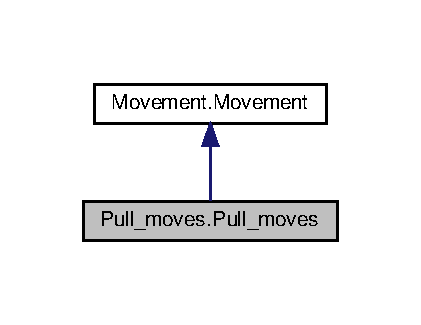
\includegraphics[width=202pt]{classPull__moves_1_1Pull__moves__inherit__graph}
\end{center}
\end{figure}


Collaboration diagram for Pull\+\_\+moves.\+Pull\+\_\+moves\+:
\nopagebreak
\begin{figure}[H]
\begin{center}
\leavevmode
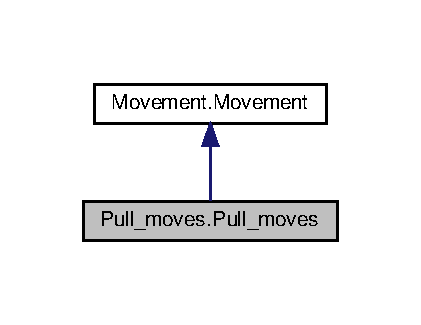
\includegraphics[width=202pt]{classPull__moves_1_1Pull__moves__coll__graph}
\end{center}
\end{figure}
\subsection*{Public Member Functions}
\begin{DoxyCompactItemize}
\item 
def \hyperlink{classPull__moves_1_1Pull__moves_a58ef6f3a1397cc435cd186513562f0a5}{mutation} (self, structure\+\_\+grid)
\item 
def \hyperlink{classPull__moves_1_1Pull__moves_a6456567c18974da96c3c8bbbca78b989}{\+\_\+\+\_\+init\+\_\+\+\_\+} (self, res, i)
\end{DoxyCompactItemize}
\subsection*{Public Attributes}
\begin{DoxyCompactItemize}
\item 
\mbox{\Hypertarget{classPull__moves_1_1Pull__moves_aa85e15fa4b93a732a2015e3e5f9e8002}\label{classPull__moves_1_1Pull__moves_aa85e15fa4b93a732a2015e3e5f9e8002}} 
{\bfseries residu}
\end{DoxyCompactItemize}


\subsection{Detailed Description}
\begin{DoxyVerb}A square is formed by residues i, i + 1, L and C.
    A pull move can only proceed if C is either empty or occupied by residue i - 1.
\end{DoxyVerb}
 

\subsection{Constructor \& Destructor Documentation}
\mbox{\Hypertarget{classPull__moves_1_1Pull__moves_a6456567c18974da96c3c8bbbca78b989}\label{classPull__moves_1_1Pull__moves_a6456567c18974da96c3c8bbbca78b989}} 
\index{Pull\+\_\+moves\+::\+Pull\+\_\+moves@{Pull\+\_\+moves\+::\+Pull\+\_\+moves}!\+\_\+\+\_\+init\+\_\+\+\_\+@{\+\_\+\+\_\+init\+\_\+\+\_\+}}
\index{\+\_\+\+\_\+init\+\_\+\+\_\+@{\+\_\+\+\_\+init\+\_\+\+\_\+}!Pull\+\_\+moves\+::\+Pull\+\_\+moves@{Pull\+\_\+moves\+::\+Pull\+\_\+moves}}
\subsubsection{\texorpdfstring{\+\_\+\+\_\+init\+\_\+\+\_\+()}{\_\_init\_\_()}}
{\footnotesize\ttfamily def Pull\+\_\+moves.\+Pull\+\_\+moves.\+\_\+\+\_\+init\+\_\+\+\_\+ (\begin{DoxyParamCaption}\item[{}]{self,  }\item[{}]{res,  }\item[{}]{i }\end{DoxyParamCaption})}

\begin{DoxyVerb}Initialize the object End_moves
    :param res: Residu object
    :param   i: index of the Residu object
\end{DoxyVerb}
 

\subsection{Member Function Documentation}
\mbox{\Hypertarget{classPull__moves_1_1Pull__moves_a58ef6f3a1397cc435cd186513562f0a5}\label{classPull__moves_1_1Pull__moves_a58ef6f3a1397cc435cd186513562f0a5}} 
\index{Pull\+\_\+moves\+::\+Pull\+\_\+moves@{Pull\+\_\+moves\+::\+Pull\+\_\+moves}!mutation@{mutation}}
\index{mutation@{mutation}!Pull\+\_\+moves\+::\+Pull\+\_\+moves@{Pull\+\_\+moves\+::\+Pull\+\_\+moves}}
\subsubsection{\texorpdfstring{mutation()}{mutation()}}
{\footnotesize\ttfamily def Pull\+\_\+moves.\+Pull\+\_\+moves.\+mutation (\begin{DoxyParamCaption}\item[{}]{self,  }\item[{}]{structure\+\_\+grid }\end{DoxyParamCaption})}

\begin{DoxyVerb}text
\end{DoxyVerb}
 

The documentation for this class was generated from the following file\+:\begin{DoxyCompactItemize}
\item 
Pull\+\_\+moves.\+py\end{DoxyCompactItemize}

\hypertarget{classResidu_1_1Residu}{}\section{Residu.\+Residu Class Reference}
\label{classResidu_1_1Residu}\index{Residu.\+Residu@{Residu.\+Residu}}
\subsection*{Public Member Functions}
\begin{DoxyCompactItemize}
\item 
def \hyperlink{classResidu_1_1Residu_a2c2303a44077b9baff5d95cf80de3619}{search\+\_\+free\+\_\+neighbour} (self, structure\+\_\+grid)
\item 
\mbox{\Hypertarget{classResidu_1_1Residu_a07b258a1c699616ec59d4224283b398d}\label{classResidu_1_1Residu_a07b258a1c699616ec59d4224283b398d}} 
def {\bfseries \+\_\+\+\_\+init\+\_\+\+\_\+} (self, hydrophobicity, x, y)
\end{DoxyCompactItemize}
\subsection*{Public Attributes}
\begin{DoxyCompactItemize}
\item 
\mbox{\Hypertarget{classResidu_1_1Residu_af778501a86dc7d49803784c36fadecaf}\label{classResidu_1_1Residu_af778501a86dc7d49803784c36fadecaf}} 
{\bfseries hp}
\item 
\mbox{\Hypertarget{classResidu_1_1Residu_a52fde1932f96aac85f7fc3085ecf2409}\label{classResidu_1_1Residu_a52fde1932f96aac85f7fc3085ecf2409}} 
{\bfseries line}
\item 
\mbox{\Hypertarget{classResidu_1_1Residu_a8f226a0502f5490c82c0a01c10bfcb01}\label{classResidu_1_1Residu_a8f226a0502f5490c82c0a01c10bfcb01}} 
{\bfseries column}
\end{DoxyCompactItemize}


\subsection{Detailed Description}
\begin{DoxyVerb}text
\end{DoxyVerb}
 

\subsection{Member Function Documentation}
\mbox{\Hypertarget{classResidu_1_1Residu_a2c2303a44077b9baff5d95cf80de3619}\label{classResidu_1_1Residu_a2c2303a44077b9baff5d95cf80de3619}} 
\index{Residu\+::\+Residu@{Residu\+::\+Residu}!search\+\_\+free\+\_\+neighbour@{search\+\_\+free\+\_\+neighbour}}
\index{search\+\_\+free\+\_\+neighbour@{search\+\_\+free\+\_\+neighbour}!Residu\+::\+Residu@{Residu\+::\+Residu}}
\subsubsection{\texorpdfstring{search\+\_\+free\+\_\+neighbour()}{search\_free\_neighbour()}}
{\footnotesize\ttfamily def Residu.\+Residu.\+search\+\_\+free\+\_\+neighbour (\begin{DoxyParamCaption}\item[{}]{self,  }\item[{}]{structure\+\_\+grid }\end{DoxyParamCaption})}

\begin{DoxyVerb}Search for freedom neighbour and return a dictionnaire
    of their coordinates
\end{DoxyVerb}
 

The documentation for this class was generated from the following file\+:\begin{DoxyCompactItemize}
\item 
Residu.\+py\end{DoxyCompactItemize}

%--- End generated contents ---

% Index
\backmatter
\newpage
\phantomsection
\clearemptydoublepage
\addcontentsline{toc}{chapter}{Index}
\printindex

\end{document}
